%%%%%%%%%%%%%%%%%%%%%%%%%%%%%%%%%%%%%%%%%
% Beamer Presentation
% LaTeX Template
% Version 1.0 (10/11/12)
%
% This template has been downloaded from:
% http://www.LaTeXTemplates.com
%
% License:
% CC BY-NC-SA 3.0 (http://creativecommons.org/licenses/by-nc-sa/3.0/)
%
%%%%%%%%%%%%%%%%%%%%%%%%%%%%%%%%%%%%%%%%%
\documentclass{beamer}

\mode<presentation> {
\usetheme{Madrid}
\usefonttheme{serif} 
\setbeamertemplate{navigation symbols}{} 
}
\usepackage{graphicx} % Allows including images
\usepackage{booktabs} % Allows the use of \toprule, \midrule and \bottomrule in tables
\usepackage[T1]{fontenc}
\usepackage[utf8]{inputenc}
\usepackage{amsmath}
\usepackage{color}
%\usepackage[czech]{babel}
\usepackage{lmodern}  
\usepackage{rotating}
\usepackage{scrextend}
\usepackage{pifont}
\usepackage{hyperref}
\usepackage{bm}
%----------------------------------------------------------------------------------------
%	TITLE PAGE
%----------------------------------------------------------------------------------------

\title[Týden 5]{Praktikum z ekonometrie} % The short title appears at the bottom of every slide, the full title is only on the title page

\author{VŠE Praha} % Your name
\institute[4EK417] % Your institution as it will appear on the bottom of every slide, may be shorthand to save space
{
% Your institution for the title page
\medskip
\textit{Tomáš Formánek} % Your email address
}
\date{} % Date, can be changed to a custom date

\begin{document}

\begin{frame}
\titlepage % Print the title page as the first slide
\end{frame}

\begin{frame}
\frametitle{Outline} % Table of contents slide, comment this block out to remove it
\tableofcontents % Throughout your presentation, if you choose to use \section{} and \subsection{} commands, these will automatically be printed on this slide as an overview of your presentation
\end{frame}
%	PRESENTATION SLIDES
%---------------------------------------------------------------------
\section{Introduction}
\begin{frame}{Introduction}
\end{frame}
%---------------------------------------------------------------------
\begin{frame}{Introduction - spatial analysis}
\begin{figure}
	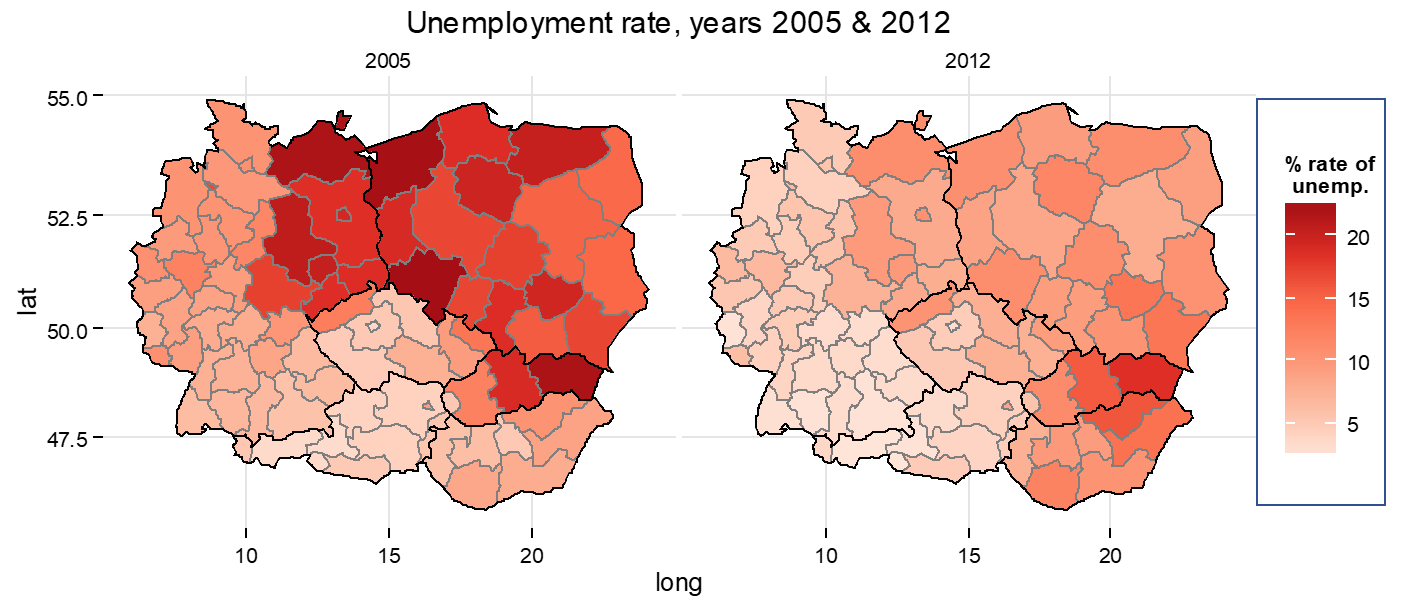
\includegraphics[width=.9\textwidth]{IMG/sp_auto2.PNG}
\end{figure}
\end{frame}
%---------------------------------------------------------------------
\begin{frame}{Introduction - spatial analysis}
Methods of quantitative spatial analysis:\\
\bigskip
\begin{itemize}
    \item Visualization \\Maps, graphical display
    \bigskip
    \item Data exploration \& descriptive methods \\Tools to broadly look at spatial patterns
    \bigskip
    \item Econometric modeling \\Fitting models, testing hypotheses, formalizing spatial dependence, discerning spatial effects from other factor (e.g. macroeconomic)
\end{itemize}
\end{frame}
%---------------------------------------------------------------------
\begin{frame}{Introduction - spatial analysis}
 What are spatial data?\\
\bigskip
\begin{itemize}
    \item Data that are location speciffic and that vary in space.
    \medskip
    \item Referenced by a spatial location $\bm{s}$ (usually 2D),  \\$\bm{s} = (x; y)$; $x$ is longitude (easting) and $y$ is latitude (northing). \\ \medskip
    May also be referenced by a zip code, county or state ID.
    \medskip
    \item Data that are close together in space (time) are often more alike than those that are far apart.
    \medskip
    \item Tobler's first law of geography: \\ ``Everything is related to everything else, but near things are more related than distant things.''
\end{itemize}
\end{frame}
%---------------------------------------------------------------------
\begin{frame}{History of spatial analysis: 1854 -- London -- cholera}
\vspace{-0.5cm}
\begin{figure}
	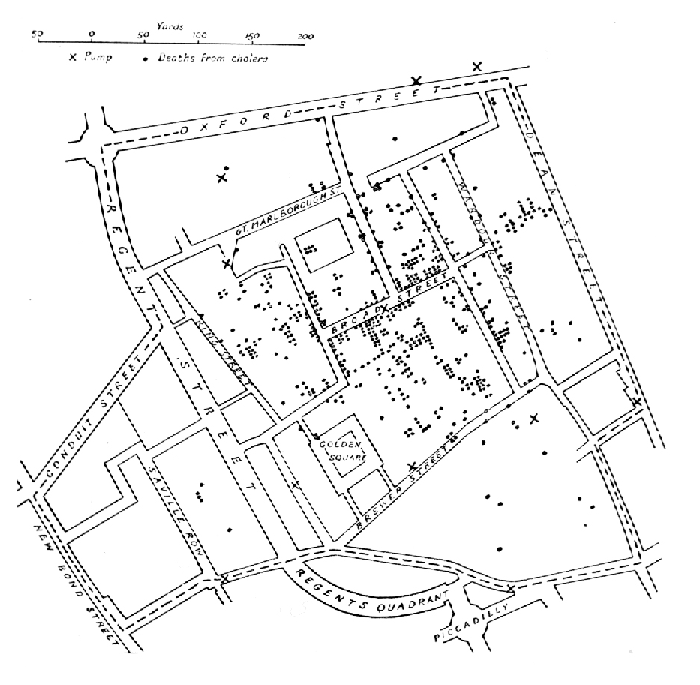
\includegraphics[width=.65\textwidth]{IMG/sp_cholera.eps}
\end{figure}
\end{frame}
%---------------------------------------------------------------------
\begin{frame}{History of spatial analysis: 1854 -- London -- cholera}
 Dr. John Snow: Early spatial analysis\\
\medskip
\begin{itemize}
    \item In August 1854, there was a major Cholera outbreak in the Soho neighbourhood of London, UK. There were 127 cholera related deaths around the area.
    \smallskip
    \item At the time, germ theory (microorganisms causing disease) was not generally accepted. Dr. J. Snow was a MD, pioneer of germ theory and a statistician.
    \smallskip
    \item Dr. John Snow spoke to local residents and mapped where cholera cases occurred. As a result of his map, he was able to pinpoint the public water pump on Broad Street as the source of contaminated water causing the cholera outbreak.
    \smallskip
    \item Dr. Snow used statistics to find a relationship between water sources and cholera cases and subsequently found out that the waterworks company supplying water to Broad Street pump was taking water from a sewage polluted area of the Thames river.
\end{itemize}
\end{frame}
%---------------------------------------------------------------------
\begin{frame}{History of spatial analysis: 1935 -- field experiments}
\vspace{-0.5cm}
\begin{figure}
	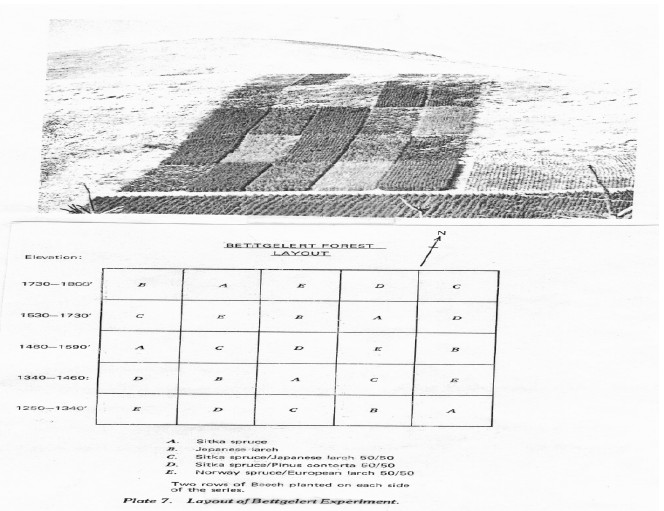
\includegraphics[width=.8\textwidth]{IMG/sp_Fisher.jpg}
\end{figure}
\end{frame}
%---------------------------------------------------------------------
\begin{frame}{History of spatial analysis: 1935 -- field experiments}
 R.A. Fisher: Early spatial analysis\\
\medskip
\begin{itemize}
    \item R.A. Fisher was probably the first to recognize implications of spatial dependency for statistical analysis.
    \smallskip
    \item In his work on design of experiments in agricultural science, he wrote (Fisher, 1935, p. 66):\\
    ``After choosing the area we usually have no guidance beyond the widely verified fact that patches in close proximity are commonly more alike, as judged by the yield of crops, than those which are further apart.''
    \smallskip
    \item Observed spatial variability, i.e. field-to-field variability, was largely due to physical properties of the soil and environmental properties of the field. He avoided the confounding of treatment effects with plot effect with the introduction of randomization.
    \smallskip
    \item Fisher's solution was to eliminate spatial dependency bias by localizing the crops under scrutiny into randomly assigned blocks.
\end{itemize}
\end{frame}
%---------------------------------------------------------------------
\section{Spatial stochastic processes}
\begin{frame}{Spatial stochastic processes}
\end{frame}
%---------------------------------------------------------------------
\begin{frame}{Measuring spatial variables}
Spatial data: measurements and measurement scales
\begin{itemize}
    \item \textbf{Generally, data vary continuously over space, but are measured only at discrete locations.} 
    \begin{itemize}
        \item To characterize spatial variables, spatial aggregation is necessary.
        \item Aggregation of spatial variables may be just another source of bias and potential data mis-manipulation\\ 
        Summary values are influenced by shape and scale of spatial units.\\
        Shape (administrative boundaries) may change over time.
    \end{itemize}
    \item Scale, consistency and relevance should be carefully considered
when collecting and analyzing spatial data
\end{itemize}
\medskip
Spatio-temporal data:
\begin{itemize}
    \item Data that are location specific and repeated in time.
    \item Each variable-observation has a location, time and value.
    \item Similar methods for analysis, with an added time dimension \\(choice of sampling frequency, spatial panel data analysis)
\end{itemize}
\end{frame}
%---------------------------------------------------------------------
\begin{frame}{Measuring spatial distances}
Distances ($d$) can be defined in a variety of ways, yet the following technical conditions should always apply (invariant to spatial translation, i.e. ``shift''):\\
\medskip
\begin{enumerate} 
\item[1] $d(\bm{s}_i, \bm{s}_j) = d(\bm{s}_j, \bm{s}_i)$ \\ \smallskip (symmetry) 
\medskip
\item[2] $d(\bm{s}_i, \bm{s}_i) = 0$  \\ \smallskip (dist. between a point and itself is zero) 
\medskip
\item[3] $d(\bm{s}_i, \bm{s}_j) \leq d(\bm{s}_i) + d(\bm{s}_j)$  \\ \smallskip (triangle inequality; 
$d(\bm{s}_i)$ is the distance from origin) 
\end{enumerate}
\end{frame}
%---------------------------------------------------------------------
\begin{frame}{Measuring spatial distances}
\small{\textbf{Euclidean distances}, measured between two point in the ``ordinary'' Euclidean space. In 2D, the Euclidean distance ($L_2$ norm) is defined as 
$$
d(\bm{s}_i, \bm{s}_j) = \sqrt[]{(s_{ix}-s_{jx})^2+(s_{iy}-s_{jy})^2}\,,
$$
where the $x$ and $y$ subscripts handle planar coordinates. For smaller distances, the computational simplicity is attractive.\\
\medskip
\textbf{Great circle distances} - for larger distances, planar projection accumulates non-negligible errors. The shortest path between two points on a sphere (given their longitudes and latitudes): 
$$
d(\bm{s}_i, \bm{s}_j) = 2r \, \arcsin \,
 \sqrt{ \sin^2 \left( \frac{\phi_j-\phi_i}{2} \right)
       + \cos(\phi_i) \cos(\phi_j)
       \sin^2 \left( \frac{l_j-l_i}{2} \right) }\,,
$$
where $r$ is the radius of the sphere, $\phi_1$ and $\phi_2$ are the latitudes of $\bm{s}_i$ and $\bm{s}_j$ in radians, $l_i$ and $l_j$ are the longitudes (in radians). Its only an approximation when applied to the Earth, which is not a perfect sphere (correct within a 0.5\%; alternative: Vicenty's formulae).\\
\medskip
\textbf{Manhatan distances} - $L_1$ norm, a function on a fixed grid.
}
\end{frame}
%---------------------------------------------------------------------
\begin{frame}{Spatial stochastic processes}
For a generic location $\bm{s}$ given by a vector of $d$ coordinates in a $d$-dimensional Euclidean space, spatial stochastic process \\(``random field'') is often denoted as
$$ Z(\bm{s}): \bm{s} \in D \subseteq \mathbb{R}^d \, .$$
\vspace{-0.5cm}
\begin{itemize}
    \item Typically, $d=2$ for most economic and econometric applications, $d=3$ is often used in fields such as geology or astronomy. 
    \smallskip
    \item $D$ is a fixed finite set of $N$ spatial locations $\bm{s}_1, \bm{s}_2, \dots, \bm{s}_N$. 
    \smallskip
    \item Individual $\bm{s}_i$ units are points in space (say, with GPS-based latitude and longitude coordinates). Sometimes, such points can be associated with non-zero surface area elements.
    \item Much like in time-series analysis, the individual realizations of a spatial stochastic process -- random field -- are often denoted \\$z(\bm{s}_i)$ or, simply, $z_i$.
\end{itemize}
\end{frame}
%---------------------------------------------------------------------
\begin{frame}{Spatial stochastic processes}
Stationarity is a common assumption: a spatial process under scrutiny repeats itself over the domain $D$. If we translate the entire set of coordinates by $\bm{h}$ -- a specific distance in a specified direction, the stochastic process and its features remain unchanged.\\
\medskip
\textbf{Strong stationarity} of a random filed: We start with a finite-dimensional distribution: 
$$F_{\bm{s}_1, \dots,\bm{s}_m }(z_1,\dots, z_m) = P[Z(\bm{s}_1) \leq z_1, Z(\bm{s}_2) \leq z_2, \dots, Z(\bm{s}_m) \leq z_m] \, .$$  
Strong stationarity $\leftrightarrow$~$F$ is invariant under spatial translation $\bm{h}$. Unlike $d_{ij}$ (Euclidean distance between two spatial units $\bm{s}_i$ and $\bm{s}_j$), \\$\bm{h}$ is an orientated distance ``shift'' (spatial translation) vector. \\For strong stationarity:
\begin{equation*}
\begin{aligned}
& P \left[Z(\bm{s}_1) \leq z_1, Z(\bm{s}_2) \leq z_2, \dots, Z(\bm{s}_m) \leq z_m \right] \\
& = P \left[Z(\bm{s}_1+\bm{h}) \leq z_1, Z(\bm{s}_2+\bm{h}) \leq z_2, \dots, Z(\bm{s}_m+\bm{h}) \leq z_m \right] \, .
\end{aligned} 
\end{equation*}
\end{frame}
%---------------------------------------------------------------------
\begin{frame}{Spatial stochastic processes}
\vspace{-0.2cm}
\textbf{Weak  stationarity} (also called second order stationarity) assumes that the first two moments exist, are invariant (and finite) and covariance only depends on spatial translation (orientated distance) $\bm{h}$:
\begin{equation*}
\begin{aligned}  
E[Z(\bm{s})] &= \mu \,, \\
\textnormal{var}[Z(\bm{s})] & = \sigma^2 \,, \\
\textnormal{cov} [Z(\bm{s}+\bm{h}),Z(\bm{s})] = C(\bm{s}+\bm{h}, \bm{s}) & = C(\bm{h}) \,.
\end{aligned} 
\end{equation*}
As autocovariance is a function of $\bm{h}$ only (under weak st.), \\for any spatial points $\bm{s}_i$ and $\bm{s}_j$ such that $\bm{s}_i -\bm{s}_j = \bm{h}$, we can write: 
\begin{equation*}
\textnormal{cov} \left[ Z(\bm{s}_i), Z(\bm{s}_j) \right] = C(\bm{s}_i - \bm{s}_j) = C(\bm{h}) \,.  
\end{equation*}
Covariogram $C(\bm{h})$ is the covariance between two spatial units, separated by $\bm{h}$. For $\bm{h} = \bm{0}$, it simply describes variance: 
$$\textnormal{cov}\,[Z(\bm{s}+\bm{0}),Z(\bm{s})] =  C(\bm{0}) = \textnormal{var}\,[Z(\bm{s})]\,.$$
Under weak dependency, covariance disappears with growing distance: 
$$C(\bm{h}) \rightarrow 0~\textnormal{as}~||\bm{h}|| \rightarrow \bm{\infty}$$.
\end{frame}
%---------------------------------------------------------------------
\begin{frame}{Spatial stochastic processes}
\textbf{Intrinsic stationarity} is less restrictive than weak (second order) stationarity and it is defined in terms of first differences. \\
\smallskip
A spatial process is intrinsically stationary if the difference between two observed spatial points is weakly stationary: 
\begin{equation*} 
\begin{aligned}  
E[Z(\bm{s}+\bm{h})-Z(\bm{s})] &= 0 \,, \\
\textnormal{var}[Z(\bm{s}+\bm{h})-Z(\bm{s})] & = 2\gamma(\bm{h}) \,,
\end{aligned} 
\end{equation*}
where $2\gamma(\bm{h}) \geq 0$ is the variogram. Generally, $2\gamma(\bm{h})$ increases with growing oriented distance $\bm{h}$. \\
\smallskip
The two types of relaxed stationarity are related: weak stationarity implies intrinsic stationarity but not vice versa. For weakly stationary spatial processes (where $E(Z(\bm{s}+\bm{h}))=E(Z(\bm{s}))=\mu$) the variogram simplifies to: 
\begin{equation*}
2\gamma(\bm{h}) = E \left[ \left( Z(\bm{s}+\bm{h}) - Z(\bm{s})  \right)^2 \right],
\end{equation*}
i.e. to the expected squared difference between two observed realizations of a spatial stochastic process. 
\end{frame}
%---------------------------------------------------------------------
\begin{frame}{Spatial stochastic processes}
\textbf{Semivariogram} is denoted as $\gamma(\bm{h})$ and it equals to half the variogram. \\ \smallskip Since  $2\gamma(\bm{h})$ is calculated as expectation of a square, $\gamma(\bm{h}) \geq 0$ for both weakly and intrinsically stationary random fields. \\ \smallskip Also, at $\bm{h}=\bm{0}$, $\gamma(\bm{0}) = 0$ because 
$$ E \left[ \left( Z(\bm{s}_i) - Z(\bm{s}_i)  \right)^2 \right]=0 \textnormal{~for~} \forall \, i\,.$$
Variogram (semivariogram) is a generalization of the covariogram $C(\bm{h})$ and under weak stationarity, the two functions are related by: 
\begin{equation*}
    \gamma(\bm{h}) = C(\bm{0}) - C(\bm{h})\,.
\end{equation*}
If a stationary stochastic process has no spatial dependency at all \\(i.e. $C(\bm{h})=0$ for $\bm{h}\not =\bm{0}$), the semivariogram is constant: $\gamma(\bm{h}) = \textnormal{var}[Z(\bm{s})]$ everywhere, except for $\bm{h}=\bm{0}$, where $\gamma(\bm{0})=0$. 
\end{frame}
%---------------------------------------------------------------------
\begin{frame}{Spatial stochastic processes}
\textbf{Isotropic spatial process} may be defined through a semivariogram:\\  $$\gamma(\bm{h})=\gamma(||\bm{h}||)=\gamma(d).$$ 
Isotropy means that the semivariogram depends only on the distance $d$ between two points and not on direction.\\ \medskip The lack of isotropy -- anisotropy -- means the semivariogram depends on direction as well as distance. \\ \medskip To assess and test anisotropy, we can estimate and plot directional semivariograms (shown next).
\end{frame}
%---------------------------------------------------------------------
\begin{frame}{Spatial stochastic processes}
\textbf{Empirical semivariogram} \\
To perform empirical analysis of distance-based data correlations, we construct the so called empirical semivariogram. First, we divide the distances observed over the domain $D$ into $K$ conveniently chosen intervals: 
$$I_1 = (0, d_1 ], \, I_2 = (d_1, d_2 ], \, \dots \, , \, I_K = (d_{K-1}, d_K ] \, .$$
Here, $d_1$ is the maximum distance within the $I_1$ interval and $d_K$ is the maximum distance observed over the field of data. \\ \smallskip The intervals can be proportional in terms of distance or in terms of sets of observation pairs allocated to each interval (to adjust for unevenly spaced observations). \\ \smallskip Note that distances are determined by $d$ (distance magnitudes) only -- here, we do not use the orientated distances $\bm{h}$.
\end{frame}
%---------------------------------------------------------------------
\begin{frame}{Spatial stochastic processes}
\textbf{Empirical semivariogram} is calculated using the following formula:
\begin{equation*}
\hat{\gamma}(d_k) = 
\frac{1}{2N(d_k)} \sum_{N(d_k)}[Z(\bm{s}_i)-Z(\bm{s}_j)]^2 \,,
\end{equation*}
where $N(d_k)$ is the number of distinct observation pairs in the interval $I_k$ and $\hat{\gamma}(d_k)$ is the semivariogram estimate for its corresponding group (interval) of distances. \\
\bigskip
Usually, we fit a convenient parametric function (exponential, spherical, Gaussian, etc.) to the estimated $\hat{\gamma}(d_k)$ values (shown next). \\ 
\bigskip
The main goal of empirical semivariogram construction is to estimate and visualize the spatial autocorrelation structure of the observed stochastic process.
\end{frame}
%---------------------------------------------------------------------
\begin{frame}{Empirical semivariogram}
\begin{figure}
	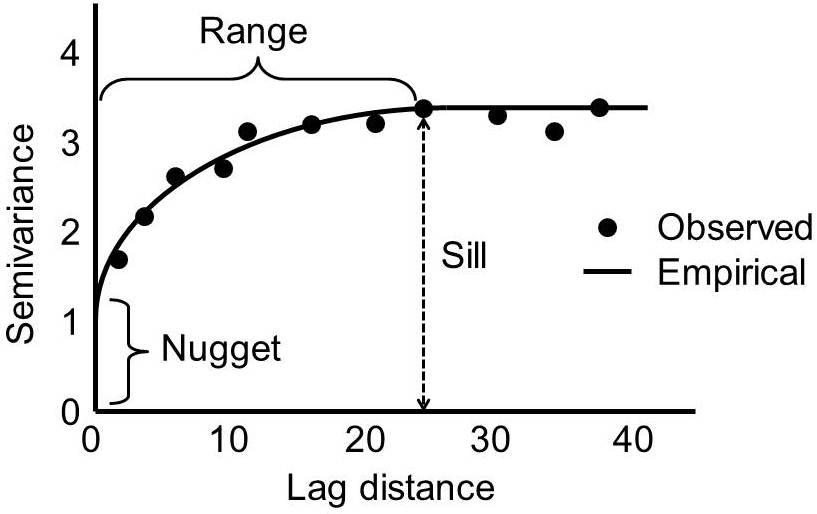
\includegraphics[width=.9\textwidth]{IMG/sp_svgm.jpg}
\end{figure}
\end{frame}
%---------------------------------------------------------------------
\begin{frame}{Empirical semivariogram}
Three main features of an estimated empirical semivariogram: 
\begin{itemize}
\item \textit{Nugget} (nugget effect) describes the micro-scale variations or measurement errors in data. Theoretically, at zero distance, $\gamma(0)=0$. However, two factors play a role here: First, $\gamma(d_1)$ is estimated over the $N(d_1)$ set of pairs, i.e. for the first interval where $ d_{ij} \in (0, d_1 ]$. Second, fitting the empirical semivariogram curve to observed values often causes the non-zero nugget.
\smallskip
\item \textit{Sill} amounts to $\lim_{d \to \infty} \gamma(d)$. The sill corresponds to variance of the stochastic field at distances where spatial dependency (which reduces $\gamma(d)$) no longer applies. $\lim_{d \to \infty} \gamma(d) = C(\bm{0}) = \textit{var}[Z(\bm{s})]$.
\smallskip
\item \textit{Range} is the spatial distance (if any) beyond which the data are not autocorrelated. In a way, range describes the strength of spatial structure -- based on where the semivariogram ``reaches'' its asymptote (sill).
\end{itemize}
\end{frame}
%---------------------------------------------------------------------
\begin{frame}{Empirical semivariogram (fitting)}
\vspace{-0.25cm}
\begin{figure}
	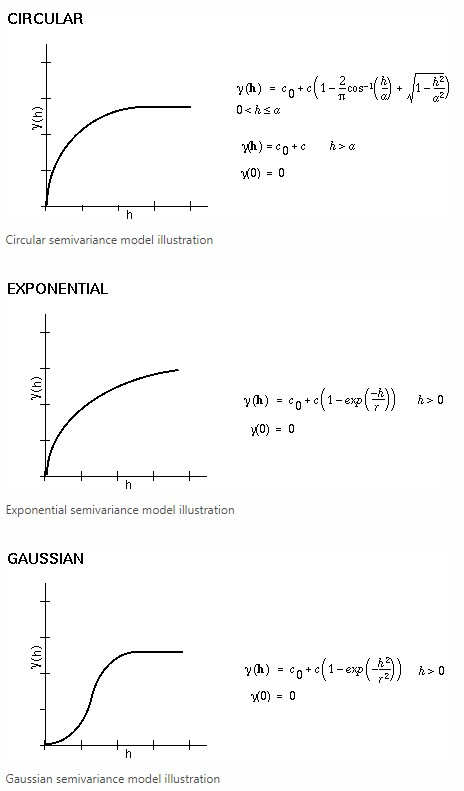
\includegraphics[width=.4\textwidth]{IMG/sp_svgm2.jpg}
\end{figure}
\end{frame}
%---------------------------------------------------------------------
\begin{frame}{Empirical semivariogram (directional semivariogram)}
\begin{figure}
	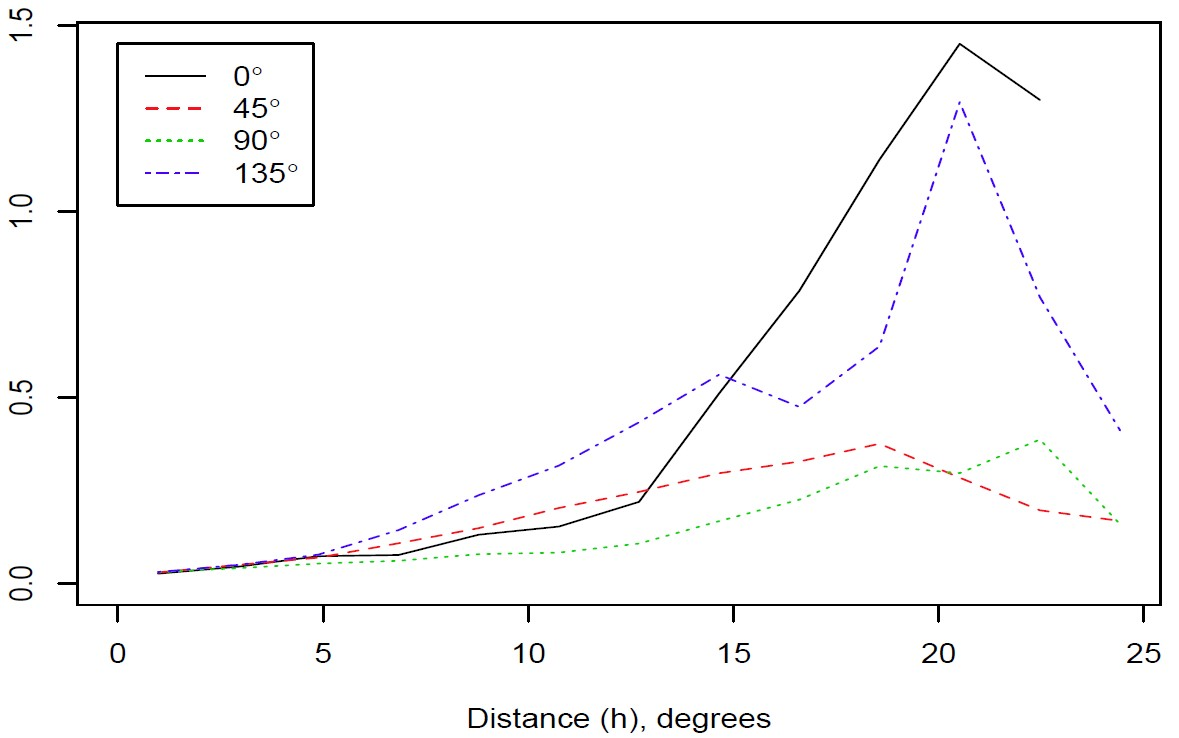
\includegraphics[width=.8\textwidth]{IMG/sp_svgm3.jpg}
\end{figure}
\end{frame}
%---------------------------------------------------------------------
\begin{frame}{Spatio-temporal stochastic processes}
The above discussion can be generalized to accommodate processes that are observed repeatedly over time. \\ \medskip 
Such observations usually exhibit both spatial and temporal dependency and variability.\\ \medskip  
Given the frequency and density limitations of empirical measurements in continuous space and time, we model our observations as realizations of a spatio-temporal random function (random field)
\begin{equation*} 
Z(\bm{s},t), \hspace{1cm} \textnormal{where~} (\bm{s},t) \in \, \mathbb{R}^d \! \times \mathbb{R} \,,
\end{equation*}
the spatio-temporal domain is indexed in space by $\bm{s} \in \mathbb{R}^d$ and in time by $t \in \mathbb{R}$. \\ \medskip 
The separation between spatial and time dimensions is substantial, which is reflected in the notation.
\end{frame}
%---------------------------------------------------------------------
\begin{frame}{Spatio-temporal stochastic processes}
Weak and intrinsic stationarity concepts can be easily expanded from spatial to spatio-temporal data. \\ \medskip
For an intrinsically stationary process $Z(\bm{s},t)$, spatio-temporal semivariograms (STSV) is:
\begin{equation*} 
\gamma(\bm{h};t) = \frac{1}{2} \textnormal{var} \left[ Z(\bm{s}_0+\bm{h} \, ; \> t_0 + t) - Z(\bm{s}_0;t_0) \right],
\hspace{1cm} (\bm{h},t) \in \, \mathbb{R}^d \! \times \mathbb{R}.
\end{equation*}
STSV does not depend on the selection of origin $(\bm{s}_0, t_0) \in \mathbb{R}^d \! \times \mathbb{R}$ (under intrinsic stationarity). \\ \medskip Also, for intrinsically stationary random fields $Z(\bm{s},t)$, the STSV $\gamma(\bm{h};t)$ is non-negative and $\gamma(\bm{0};0) = 0$.
\end{frame}
%---------------------------------------------------------------------
\begin{frame}{Empirical STSV (EU's Unemp., NUTS0, 2002---2016)}
\begin{figure}
	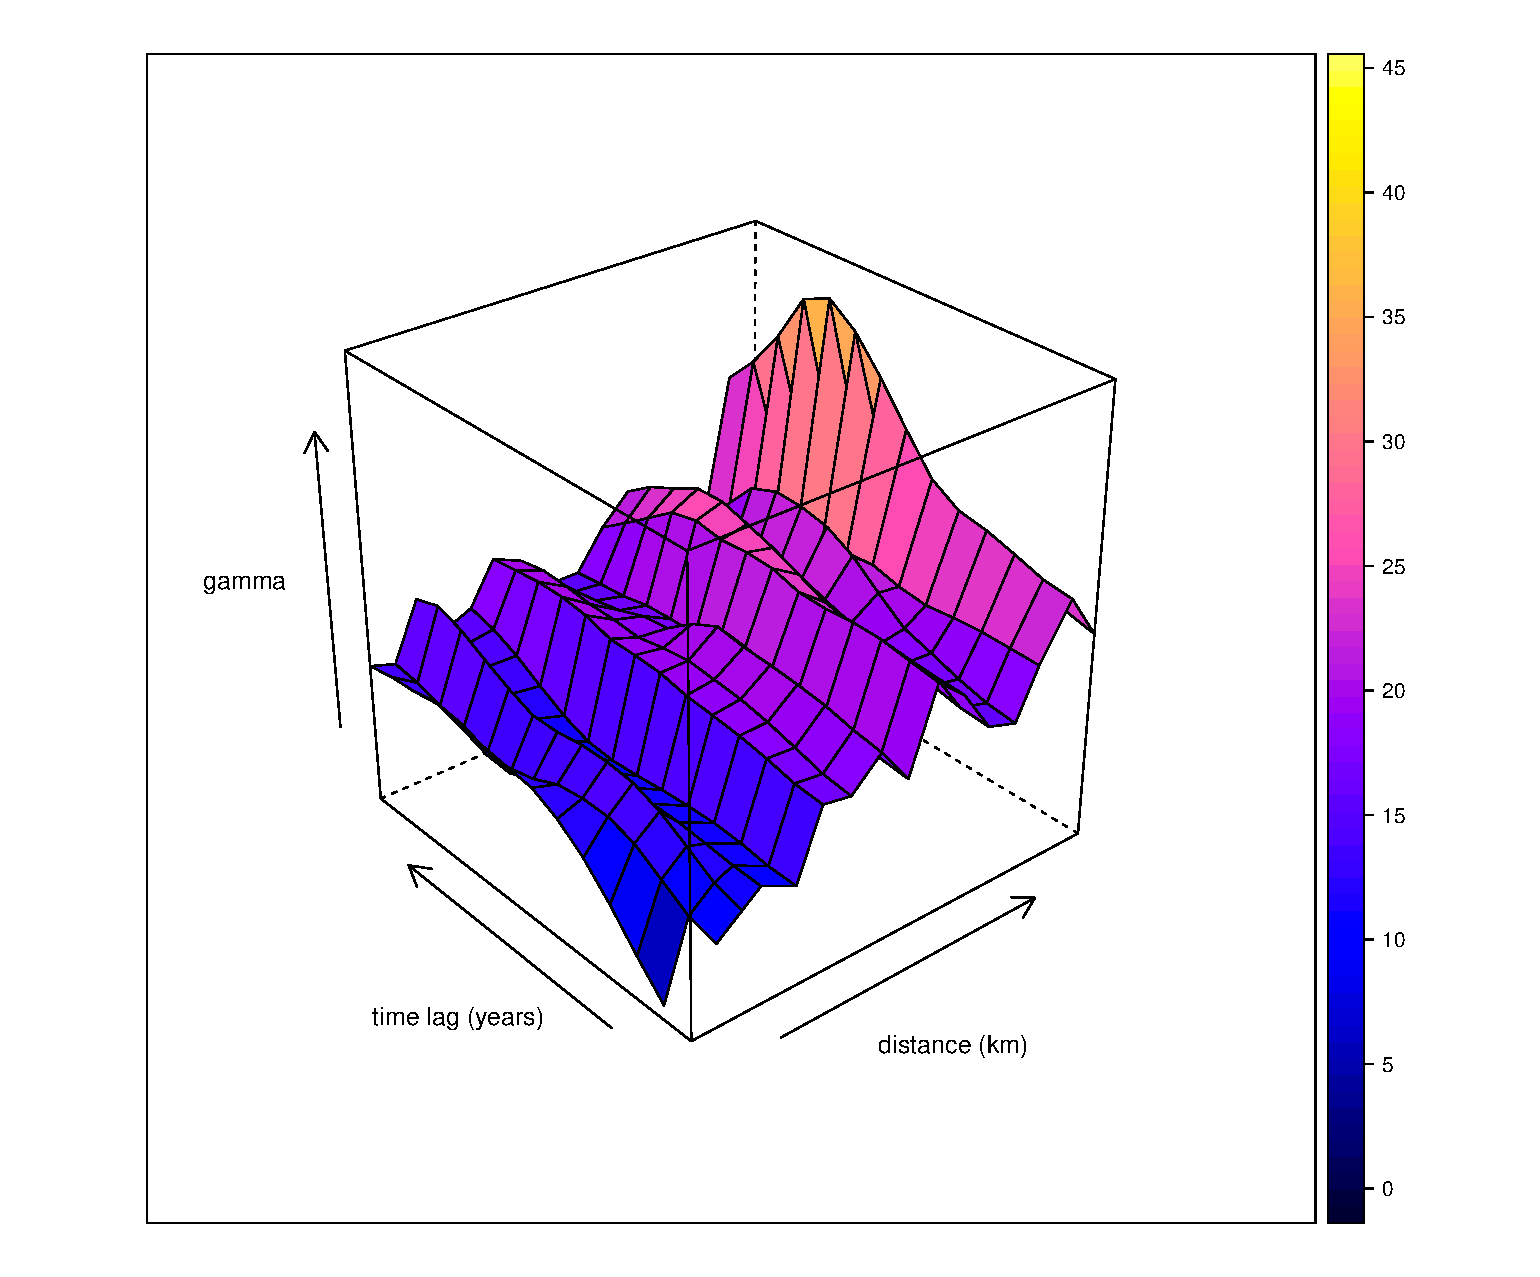
\includegraphics[width=.7\textwidth]{IMG/sp_STV.eps}
\end{figure}
\end{frame}
%---------------------------------------------------------------------
\section{Data exploration \& descriptive methods}
\begin{frame}{Data exploration \& descriptive methods}
\end{frame}
%---------------------------------------------------------------------
%\subsection{Interpolation and Krigging}
\begin{frame}{Interpolation}
\textbf{Inverse distance weighting (IDW):} a deterministic method of interpolation with a known scattered set of points. \\ \smallskip Assigned values to unknown points are calculated with a weighted average of the values available at the known points.
\\ \smallskip 
To find an interpolated value $x_0$ at a given point $\bm{s}_0$ based on samples $x_i=x(\bm{s}_i)$ with $i=1,2,\dots,N$ we use a IDW interpolating function:
$$
x(\bm{s}_0) = 
\begin{cases}
    \frac{\sum_{i=1}^N w_i(\bm{s_0})x_i}{\sum_{i=1}^N w_i(\bm{s_0})}, & 
    \textnormal{if~} d(\bm{s}_0,\bm{s}_i) \neq 0 \textnormal{~for all~}i\\
    x_i & \textnormal{if~} d(\bm{s}_0,\bm{s}_i)=0 \textnormal{~for some~}i \, 
\end{cases} 
$$
where $w_i(\bm{s}_0)=\frac{1}{d(\bm{s}_0,\bm{s}_i)^p}\,$, $\bm{s}_0$ is an interpolating (known) point, $d$ is a distance, and $p$ is a positive \textit{real} number (power parameter). \\ \smallskip
Weight decreases as distance increases from the interpolated points. High $p$ assigns greater influence to closest values -- result may turn into a mosaic of tiles (a Voronoi diagram). 
\end{frame}
%---------------------------------------------------------------------
\begin{frame}{IDW interpolation -- illustration}
\begin{figure}
	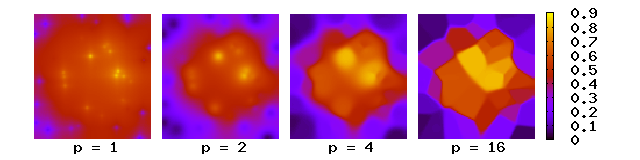
\includegraphics[width=.7\textwidth]{IMG/sp_idw.png}
\end{figure}
\end{frame}
%---------------------------------------------------------------------
\begin{frame}{Krigging}
\begin{itemize}
    \item developed by Daniel G. Krige (1919-2013) \\(originally called ``weighted moving averages'' method) 
    \smallskip
    \item Also known as BLUP (best linear unbiased prediction) and closely related to OLS estimation.
    \smallskip
    \item Returns observed values at sampling locations.
    \smallskip
    \item Interpolates values using the intensity and shape of the empirical (semi)variogram. Results depend on the choice of fitting model \\(Gaussian, spherical, exponential, etc.).
    \smallskip
    \item Uses neighborhood and/or distance search radius.
    \smallskip
    \item Provides standard errors of interpolated values.
    \smallskip
    \item Multiple approaches and generalizations exist (Block Krigging). \\
    \url{http://desktop.arcgis.com/en/arcmap/10.3/tools/3d-analyst-toolbox/how-kriging-works.htm}
\end{itemize}
\end{frame}
%---------------------------------------------------------------------
\begin{frame}{Krigging}
\textbf{Kriging}\\ \medskip
\begin{itemize}
    \item $x(\bm{s}_0)= \sum_{i=1}^N \lambda_i \, x(\bm{s}_i)$ ~~s.t.~~ $\sum_{i=1}^N \lambda_i = 1$. 
    \bigskip
    \item In IDW, $\lambda_i$ depend only on distance to the prediction location.\\
    \bigskip
    \item  With krigging, $\lambda_i$ depend on a fitted model to the measured points, the distance to the prediction location, and the spatial relationships among the measured values around the prediction location.
\end{itemize}
\end{frame}
%---------------------------------------------------------------------
\begin{frame}{Krigging -- illustration}
\begin{figure}
	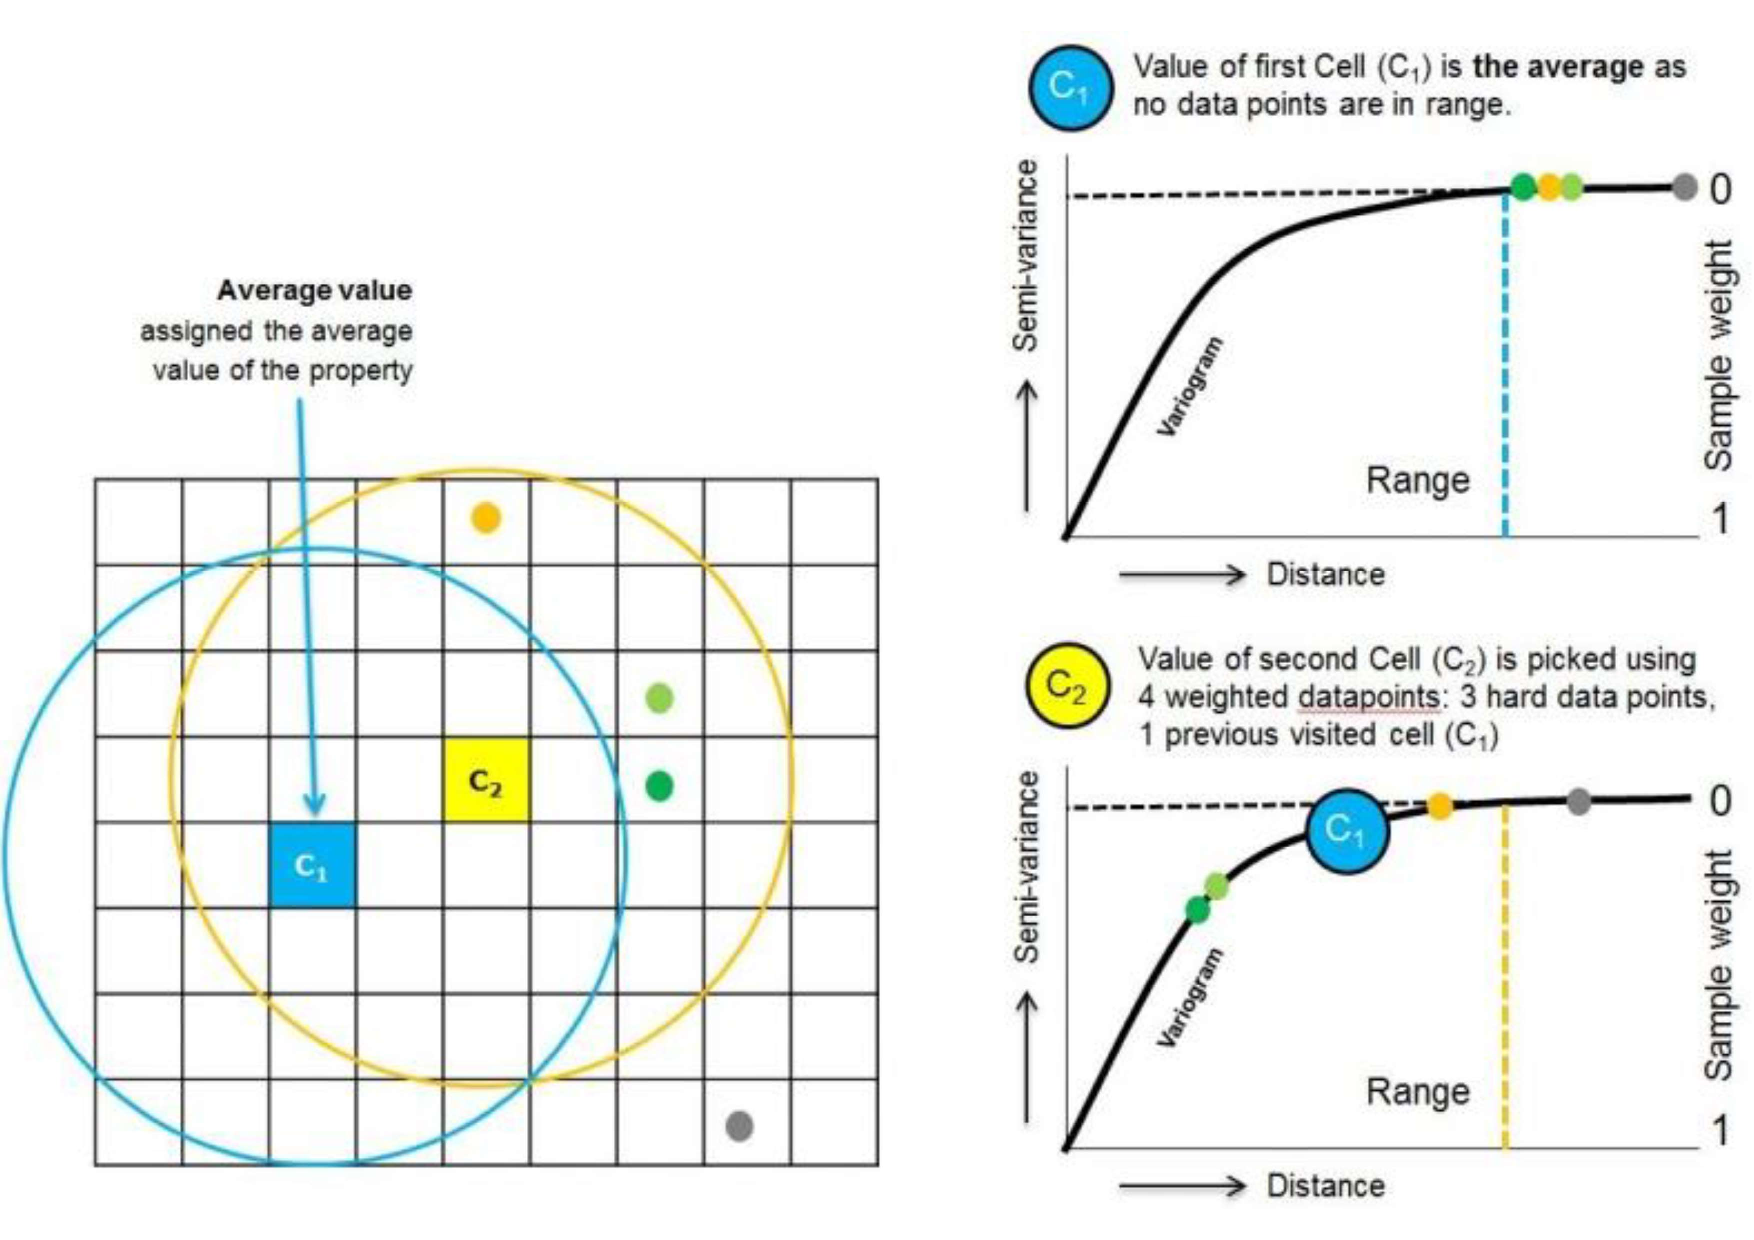
\includegraphics[width=.8\textwidth]{IMG/sp_Krigg.pdf}
\end{figure}
\end{frame}
%---------------------------------------------------------------------
\begin{frame}{Krigging}
\textbf{Ordinary kriging} assumes constant unknown mean only over the search neighborhood of $\bm{s}_{0}$. \\ \medskip
\begin{itemize}
    \item Matrix form: $x(\bm{s}_0)= \bm{\lambda}^{\prime} \, \bm{x}$ ~~s.t.~~ $\bm{\lambda}^{\prime} \bm{1} = 1$. \\
    where $\bm{\lambda}^{\prime} = (\lambda_1,\dots,\lambda_N)$ and $\bm{1}$ is a vector of ones.
    \medskip
    \item Krigging -- solve:~~~~ $\min E(x(\bm{s}_0 - \bm{\lambda}^{\prime} \, \bm{x})^2$ s.t. $\bm{\lambda}^{\prime} \bm{1} = 1$.\\
    \medskip
    \item  Minimum variance of $x(\bm{s}_0)$: $~\sigma^2= \sum_{i=1}^N \lambda_i \gamma (\bm{s}_i,\,\bm{s}_0)~+~m \,$
    \medskip
    \item is obtained when $\sum_{i=1}^N \lambda_i \gamma (\bm{s}_i,\,\bm{s}_j)~+~m = \gamma (\bm{s}_j,\,\bm{s}_0)$ for all $j$. \\
    \medskip
    Here, $\gamma$ is the semivarogram, $m$ is an additional LM parameter (mean estimate) that ensures unbiasedness of the estimate. \\For additional discussion and alternative estimation methods \\(simple, universal krigging, etc.), see\\
    \url{https://en.wikipedia.org/wiki/Kriging}
\end{itemize}
\end{frame}
%---------------------------------------------------------------------

%\subsection{Definition of neighbors}
\begin{frame}{Definition of neighbors}
\begin{itemize}
    \item Fotheringham et al (2002): ``Spatial dependency is the extent to which the value of an attribute in one location depends on the values of the attribute in nearby locations.''
    \medskip
    \item Different definitions of spatial dependency are possible.
    \medskip
    \item To discuss spatial dependency, spatial autocorrelation, corresponding tests and spatial econometric models, we need to formalize the concept of \textbf{nearby locations -- neighbors}
\end{itemize}
\end{frame}
%---------------------------------------------------------------------
\begin{frame}{Definition of neighbors}
\begin{itemize}
	\item \textbf{Distance-based approach} defines two units as neighbors if their distance does not exceed some ad-hoc predefined threshold: $\tau$. \\
	\medskip
	\begin{itemize}
		\item Can generate ``islands'' (units with zero neighbors), if $\tau$ is low compared to minimum distances among unit pairs.
		\smallskip
		\item Less suited for analysis of areas with uneven geographic density (of measurements). 
	\end{itemize}
	\medskip
	\item \textbf{Centroids} are used for measuring distances between units with non-zero areas (e.g. regions)\\
	\medskip
	\begin{itemize}
		\item Centroids can be purely geographical, ``main'' city locations, population-weighted, transportation-weighted (highway/railway), etc.
	\end{itemize}
\end{itemize}
\end{frame}
%---------------------------------------------------------------------
\begin{frame}{Definition of neighbors}
\begin{figure}
	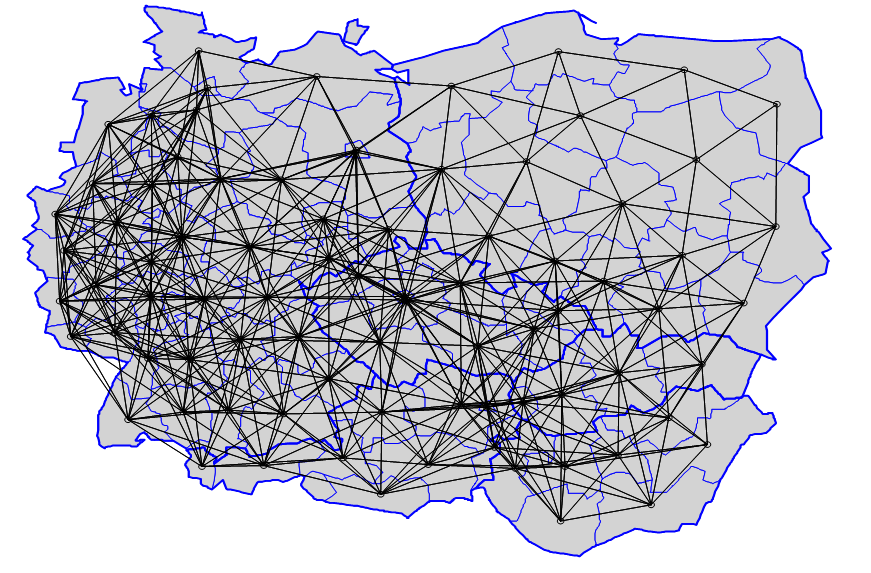
\includegraphics[width=.7\textwidth]{IMG/sp_neigb.PNG}
	\caption[]{Plot for distance-based neighbors (NUTS2), maximum neighbor distance threshold at 250 km}
\end{figure}
\end{frame}
%---------------------------------------------------------------------
\begin{frame}{Definition of neighbors}
\begin{itemize}
\item \textbf{Contiguity-based approach} spatial units (regions) are neighbors if they share a common border (at least one point).
\bigskip 
\item \textbf{Generalized contiguity approach} is based on the premise that a ``second order'' neighbor is the neighbor of a first order neighbor (the actual contiguous neighbor). \\ \smallskip With this type of approach, we can define a maximum neighborhood lag (order) to control for the highest accepted number
of neighbors traversed (not permitting cycles).	
\end{itemize}
\end{frame}
%---------------------------------------------------------------------
\begin{frame}{Definition of neighbors}
\textbf{$\bm{k}$ Nearest neighbors ($\bm{k}$NN)} \\
\medskip
For each spatial unit, we search for a preset number of $k$ nearest units that we define as its neighbors. 
\medskip
\begin{itemize}
	\item Solves for differences in areal densities ($k$ neighbors are ensured for each unit).
	\smallskip
	\item Usually leads to asymmetric spatial connectivity matrices with potentially flawed neighborhood interpretation. 
	\smallskip
	\item Illustration for $k = 3$   (neighbors only shown for 2 units):
	\begin{figure}
		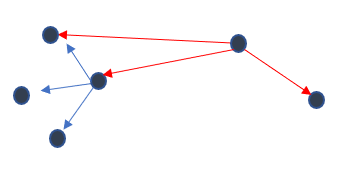
\includegraphics[width=.2\textwidth]{IMG/sp_neigb2.PNG}
	\end{figure}
\end{itemize}
\end{frame}
%---------------------------------------------------------------------
%\subsection{Spatial connectivity and weights matrices}
\begin{frame}{Spatial connectivity matrix ($\bm{C}$)}
$$
~~\bm{C} = \begin{bmatrix}
0 & 1 & 1 & 1 \\
1 & 0 & 1 & 0 \\
1 & 1 & 0 & 1 \\
1 & 0 & 1 & 0
\end{bmatrix}\quad \text{~~a 4-unit example}$$
$$c_{ij}=
	\begin{cases}
	1 & \text{if $i$ and $j$ are neighbors,}\\
	0 & \text{if $i$ and $j$ are not neighbors.}
	\end{cases}$$
\begin{itemize}
	\item Zeros on the diagonal -- units are not neighbors to themselves.
	\smallskip
	\item Spatial connectivity matrix interpretation: 
	\smallskip
	\begin{itemize}
		\item row/column 1: unit 1 is neigbor to units 2,3,4
		\item row/column 2: unit 2 is neigbor to units 1,3 (not 4)
	\end{itemize}
	\smallskip
    \item Matrix $\bm{C}$ is symmetric (for $k$NN, transformations are available).
\end{itemize}
\end{frame}
%---------------------------------------------------------------------
\begin{frame}{Spatial weights matrix ($\bm{W}$)}
\vspace{-0.5cm}
$$
\bm{C} = \begin{bmatrix}
0 & 1 & 1 & 1 \\
1 & 0 & 1 & 0 \\
1 & 1 & 0 & 1 \\
1 & 0 & 1 & 0
\end{bmatrix}\rightarrow 
\bm{W}=
\begin{bmatrix}
0 & \tfrac{1}{3} & \tfrac{1}{3} & \tfrac{1}{3} \\[2pt]
\tfrac{1}{2} & 0 & \tfrac{1}{2} & 0 \\[2pt]
\tfrac{1}{3} & \tfrac{1}{3} & 0 & \tfrac{1}{3} \\[2pt]
\tfrac{1}{2} & 0 & \tfrac{1}{2} & 0
\end{bmatrix}
$$
\begin{itemize}
	\item Usually, $\bm{W}$ is row-standadrized (to unity): 
	$w_{ij} = \frac{c_{ij}}{\sum^N_{j=1} c_{ij}}$.
	\smallskip
	\item Binary (connectivity) indicators $c_{ij}$ may be generalized prior to standardization. Hence, instead of binary $c_{ij}$, we may use inverse distances (linear, squared, \dots) -- given assumed decay in spatial dependency over distance. \\ \medskip Validity of any such prior information (decay pattern) will influence subsequent analysis (spatial dependency tests, spatial regression models).
\end{itemize}
\end{frame}
%---------------------------------------------------------------------
\begin{frame}{Spatial weights matrix ($\bm{W}$)}
\vspace{-0.2cm}
$$
\bm{W}=
\begin{bmatrix}
0 & \tfrac{1}{3} & \tfrac{1}{3} & \tfrac{1}{3} \\[2pt]
\tfrac{1}{2} & 0 & \tfrac{1}{2} & 0 \\[2pt]
\tfrac{1}{3} & \tfrac{1}{3} & 0 & \tfrac{1}{3} \\[2pt]
\tfrac{1}{2} & 0 & \tfrac{1}{2} & 0
\end{bmatrix}
$$
\begin{itemize}
	\item Each row of $\bm{W}$ ``provides'' weights for an expected value of an observed spatial variable $y_i$ -- weighted averages (fitted values) can be calculated as $\hat{\bm{y}} = \bm{Wy}$. For example:
	\begin{align*}
	\hat{y}_1 & =  \tfrac{1}{3} y_2 + \tfrac{1}{3} y_3 + \tfrac{1}{3} y_4 \\
	&\dots \\
	\hat{y}_4 & = \tfrac{1}{2} y_1  + \tfrac{1}{3} y_3 
	\end{align*}
	\item Observed values of variables can be used to predict corresponding values for neighboring spatial units.
	\smallskip
	\item In this context, $\hat{y}_i$ is often called \textit{spatial lag} of $y_i$.
\end{itemize}
\end{frame}
%---------------------------------------------------------------------
\begin{frame}{Definition of neighbors}
\vspace{-0.3cm}
\begin{figure}
	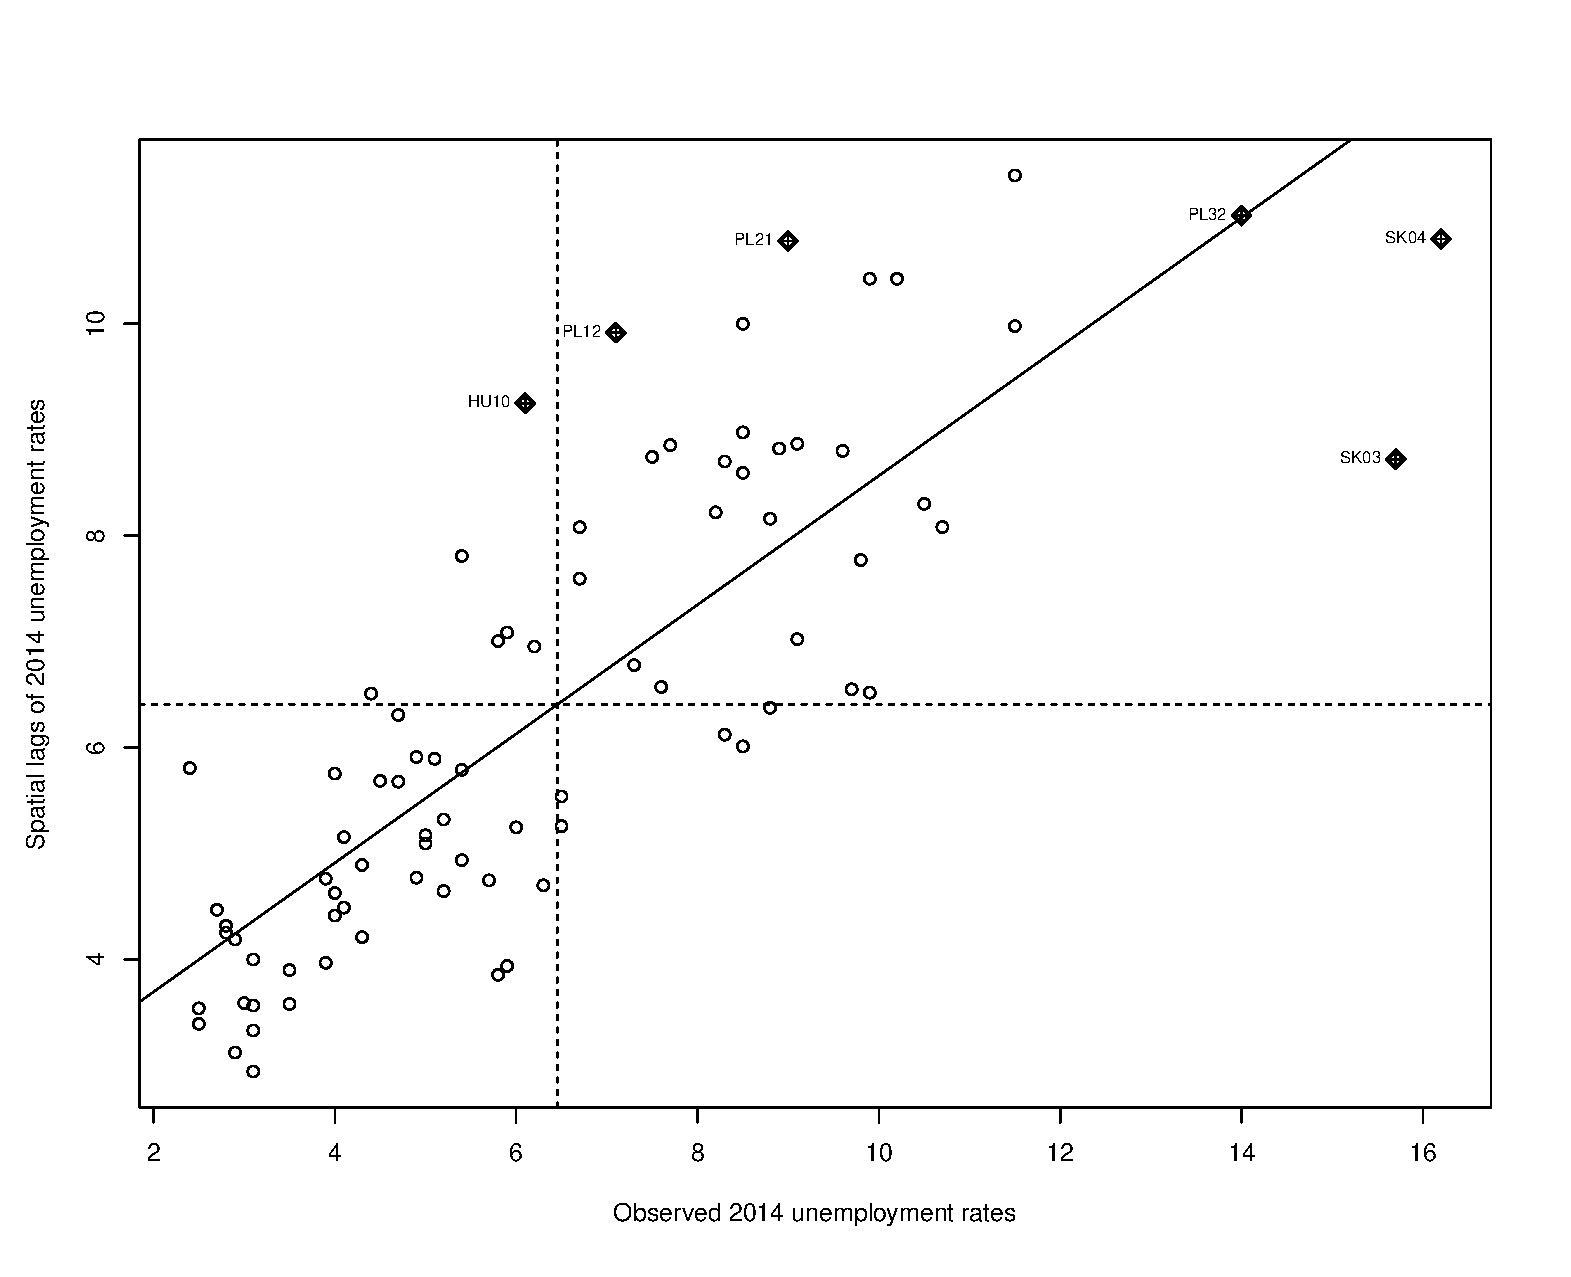
\includegraphics[width=.7\textwidth]{IMG/sp_MoranPlot.eps}
	\caption[]{Moran plot for unemployment rate, 2014, NUTS2 (AT, CZ, DE, HU, PL, SK): observed values vs. spatial lags.}
\end{figure}
\end{frame}
%---------------------------------------------------------------------
\begin{frame}{Sample selection in spatial data analysis}
\begin{itemize}
    \item Spatially autocorrelated processes are defined in terms of individual units and their interactions with neighbors. 
    \smallskip
    \item Clearly, we can only assess the impact of neighboring units if such units are part of our sample. Hence, in spatial econometrics, we usually do not draw limited samples from a particular area.
    \smallskip
    \item Instead, we work with data from adjacent units located in unbroken (``complete'') study areas.  
    \smallskip
    \item Otherwise, $\bm{C}$ and $\bm{W}$ matrices would be misleading and we could not consistently estimate spatial interactions and effects.
    \smallskip    
    \item Generally speaking, spatial analysis should include the whole geographically defined area/region instead of using random sampling (from a ``population'' of regions within the relevant area). 
\end{itemize}
\end{frame}
%---------------------------------------------------------------------
%\subsection{Spatial dependency tests}
\begin{frame}{Spatial dependency tests}
\begin{itemize}
    \item Positive spatial autocorrelation occurs if high or low values \\of a variable cluster in space. 
    \medskip
    \item For negative spatial autocorrelation, spatial units tend to be surrounded by neighbors with very dissimilar observations. 
    \medskip
    \item Spatially random data lack any spatial pattern.
    \medskip
    \item Sometimes, spatial dependency patterns are easy to discern visually using choropleths. 
    \medskip
    \item However, a formal approach towards evaluation of spatial dependency is often required.
\end{itemize}
\end{frame}
%---------------------------------------------------------------------
\begin{frame}{Moran's $I$}
Measure of global spatial autocorrelation, overall clustering of data:
\begin{equation*}
I = \frac{N}{W}\,\bm{z}'\bm{Wz}(\bm{z}'\bm{z})^{-1},
\end{equation*}     
where 
\begin{itemize}
    \item[] $N$ is the number of spatial observations (units) of the variable under scrutiny (say, $\bm{y}$),
    \smallskip
    \item[] $\bm{z}$ is the centered form of $\bm{y}$: $z_i = y_i - \bar{y}$.\\
    (Note a recast: $y_i = \beta_0 + z_i$. If SLRM is expanded by regressors, Moran's $I$ can be applied to regression residuals).
    \smallskip
    \item[] The standardization factor $W = \sum_{i}\sum_{j}w_{ij}$ corresponds to the sum of all elements of the spatial weights matrix $\bm{W}$. \\For row-standardized $\bm{W}$ matrices, $\tfrac{N}{W}=1$. Moran's $I$ can be used with $\bm{C}$ matrices (binary, generalized) as well.
\end{itemize}
\end{frame}
%---------------------------------------------------------------------
\begin{frame}{Moran's $I$}
\vspace{-0.2cm}
\begin{equation*}
I = \frac{N}{W}\,\bm{z}'\bm{Wz}(\bm{z}'\bm{z})^{-1},
\end{equation*}     
In most empirical circumstances, $I \in [ -1,1 ]$. Under the null hypothesis of spatial randomness, Moran’s $I$ is asymptotically normally distributed with the following first two moments:
\begin{equation*}
E(I) = -\frac{1}{N-1} \hspace{0.5cm} 
\textnormal{and} \hspace{0.5cm} 
\textnormal{var}(I) = \frac{N^2W_1 - NW_2 +3W^2}{(N^2-1)W^2} \,,
\end{equation*}  
where $W_1 = \sum_i \sum_j (w_{ij}+w_{ji})^2$ and $W_2 = \sum_i (\sum_j w_{ij} + \sum_j w_{ji})^2$.\\
\medskip
Normality assumption $\rightarrow$ calculate a $z$-score 
$$z=\frac{I-E(I)}{\sqrt{\textnormal{var}(I)}} $$\\
and test for statistical significance of Moran's $I$: whether neighboring units are more similar $(I > E(I))$ or more dissimilar $(I < E(I))$ than they would be under the null hypothesis of spatial randomness.
\end{frame}
%---------------------------------------------------------------------
\begin{frame}{Local Moran's $I$}
\begin{itemize}
    \item Moran's $I$ yields only one statistic that summarizes the nature of spatial dependency in the observed variable -- it assumes geographical homogeneity (stationarity) in the data. 
    \smallskip
    \item If such assumption does not hold (spatial dependency varies over space), then Moran's $I$ test loses power and the ``global'' statistic is non-descriptive. 
    \smallskip
    \item To address this problem, we can use Local Moran's $I$ statistic \\(for row-standardized $\bm{W}$):
    \begin{equation*}
    I_i = \frac{z_iN}{\bm{z}'\bm{z}}\bm{w}_{i}\bm{z} \, .
    \end{equation*}    
    \item The expected value of  Local Moran's $I$ under the null hypothesis of no spatial autocorrelation is: $E(I_i)=-w_i/(N-1)$. Here, $w_i$ is the sum of elements in the $i$-th row of $\bm{W}$.
\end{itemize}
\end{frame}
%---------------------------------------------------------------------
\begin{frame}{Local Moran's $I$}
    \begin{equation*}
    I_i = \frac{z_iN}{\bm{z}'\bm{z}}\bm{w}_{i}\bm{z} \, .
    \end{equation*}    
\begin{itemize}
    \item Values of $I_i > E(I_i)$ indicate positive spatial autocorrelation, i.e. that the $i$-th region is surrounded by regions that, on average, are similar to the $i$-th region with respect to the observed variable $y$. 
    \item $I_i < E(I_i)$ would suggest negative spatial autocorrelation.
    \item Significance of spatial dependency is then evaluated using $var(I_i)$ and the corresponding $z$-score.
    \bigskip
    \item We may see the global nature of Moran's $I$ from
    \begin{equation*} 
    I = \frac{1}{N}\sum_{i=1}^N I_{i} \,.
    \end{equation*}   
\end{itemize}
\end{frame}
%---------------------------------------------------------------------
\begin{frame}{Geary's $C$}
 Variance test similar (in principle) to the Durbin-Watson test statistic for residuals' autocorrelation in time-series regressions.
 \begin{equation*}
C = \frac{N-1}{2W}\,
    \frac{\sum_{i}\sum_{j}w_{ij}(y_i-y_j)^2}
         {\sum_{i}(y_i-\bar{y})^2} \,,
\end{equation*}   
where all elements follow from previous slides. Empirical Geary's $C$ values range from 0 to 2. However, occurrences of $C>2$ are possible.\\
\smallskip
\begin{itemize}
    \item Under the null of no spatial autocorrelation, first two moments are:
\begin{equation*}
E(C) = 1\, ,\hspace{0.5cm}
\textnormal{var}(C) = \frac{(N-1)(2W_1 + W_2) - 4W^2 }{2(N+1)W^2} \,,
\end{equation*}  
\item Positive spatial dependency: $C < 1$.\\ Negative spatial autocorrelation is reflected in $C > 1$.
\smallskip
\item $z$-transformation is asymptotically normally distributed. Therefore, $z(C)$ can be used for testing spatial randomness.
\end{itemize}
\end{frame}
%---------------------------------------------------------------------
%\subsection{Clusters -- hotspots and coldspots}
\begin{frame}{Clusters -- hotspots and coldspots}
Getis' $G^{\ast}$: spatial clusters and hotspot analysis\\
\smallskip
\begin{itemize}
    \item Clustering analysis by Getis can only be performed for positively autocorrelated spatial data.
    \smallskip
    \item $G_i^{\ast}(\tau) = \frac{\sum_{j=1}^N c_{ij}^{\ast} y_j}{\sum_{j=1}^N y_j} \,,$\\
    \smallskip
    where $c_{ij}^{\ast}$ come from amended distance-based (arbitrary $\tau$ used) connectivity matrix $\bm{C}^{\ast} = \bm{C}+\bm{I}_N$; i.e. $y_i$ observations enter $G_i^{\ast}(\tau)$ calculation. Observations of $y$ are assumed to have a natural origin and positive support.
    \smallskip
    \item $G_i^{\ast}(\tau)$ is a local stastic, a proportion of the aggregated $y_j$ values that lie within $\tau$ of $i$ to the total sum of $y_j$ observations.
    \smallskip
    \item Alternatively, Getis' statistic is calculated using $\bm{C}$ (not $\bm{C}^{\ast}$) and denoted $G_i(\tau)$ 
\end{itemize}
\end{frame}
%---------------------------------------------------------------------
\begin{frame}{Clusters -- hotspots and coldspots}
\begin{itemize}
    \item If we observe high values of $y_j$ within distance $\tau$ of unit $i$, then $G_i^{\ast}(\tau)$ would be relatively high compared to its expected value under the null hypothesis of full spatial randomness: $$E \left[G_i^{\ast}(\tau) \right] = \frac{c_i^{\ast}}{N}\,,$$ where $c_i^{\ast}$ is the sum of elements of $i$-th row of $\bm{C}^{\ast}$.
    \medskip 
    \item Also, under the $H_0$ of spatial randomness, we can write
    $$
    \textnormal{var} \left[G_i^*(\tau) \right] = 
    \frac{c_i^*(N-c_i^*)}{N^2 (N-1)}
    \left( \frac{Y_{i2}^*}{(Y_{i1}^*)^2} \right) , 
    $$ 
    where $Y_{i1}^*=\tfrac{\sum_j y_j}{N}$ and $Y_{i2}^*=\tfrac{\sum_j y_j^2}{N}-(Y_{i1}^*)^2$.
    \medskip 
    \item High positive $z$-score indicates ``hotspot'' (cluster of high values) and vice versa. Critical values provided by Getis and Ord. \\Say, for $N = 100$ and $\alpha = 5\%$, the $z$-scores would have to exceed $\pm 3.289$ for a statistically significant hot/cold spot.
\end{itemize}
\end{frame}
%---------------------------------------------------------------------
\begin{frame}{Clusters -- hotspots and coldspots}
\begin{figure}
	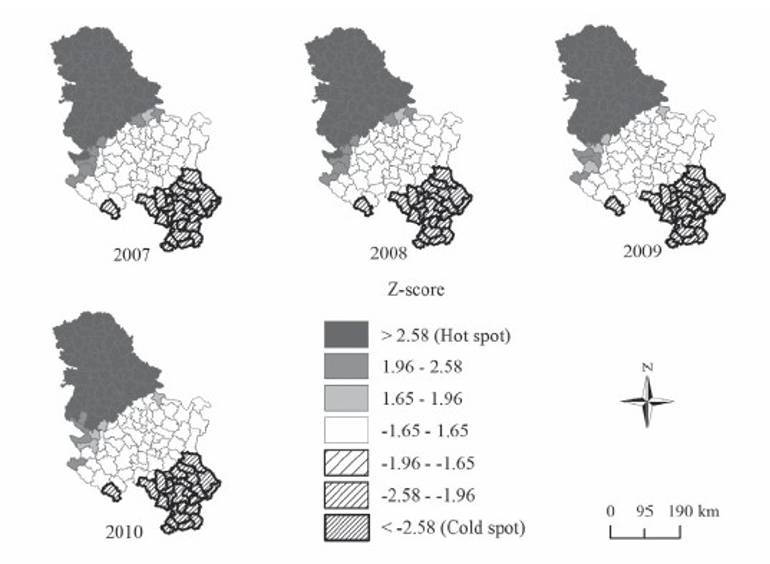
\includegraphics[width=.7\textwidth]{IMG/sp_coldspot.PNG}
	\caption{Spatial clusters (hot and cold spots) of the municipalities in Serbia by the level of average monthly net earning from 2001 to 2010}
\end{figure}
\end{frame}
%---------------------------------------------------------------------
\section{Spatial regression models}
\begin{frame}{Spatial regression models}
\end{frame}
%---------------------------------------------------------------------
\begin{frame}{Spatial regression models}
\begin{figure}
	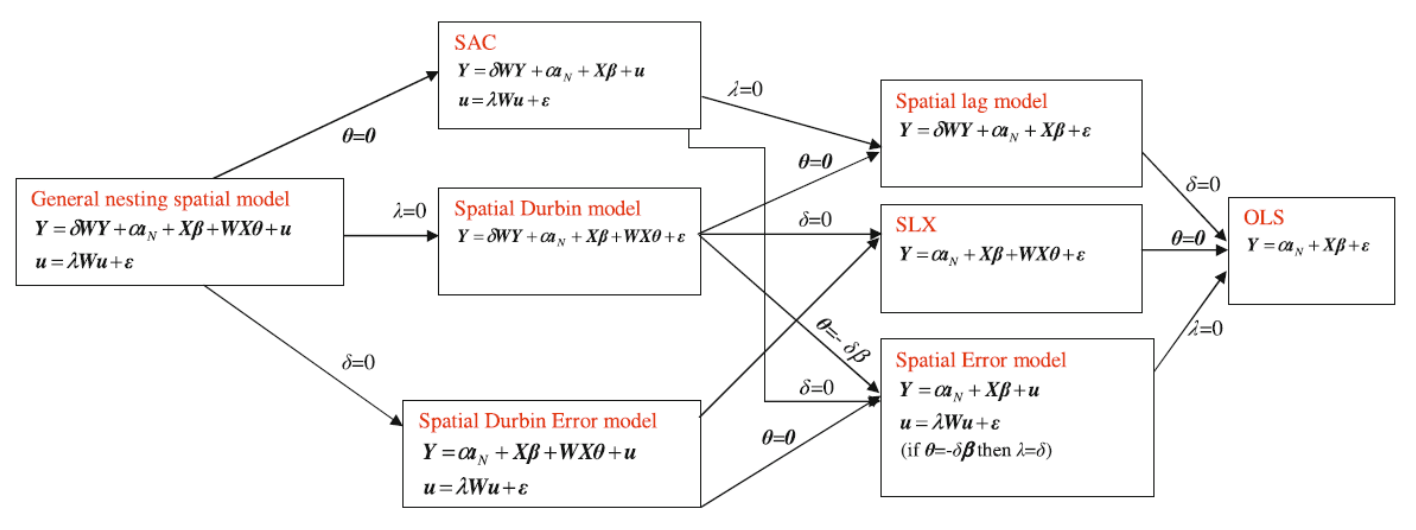
\includegraphics[width=1\textwidth]{IMG/sp_reg.PNG}
	\caption{The relationship between different spatial dependence models for cross-sectional data (source Halleck Vega and Elhorst 2012)}
\end{figure}
\end{frame}
%---------------------------------------------------------------------


\end{document}